
\begin{figure}[t!]
    \centering
    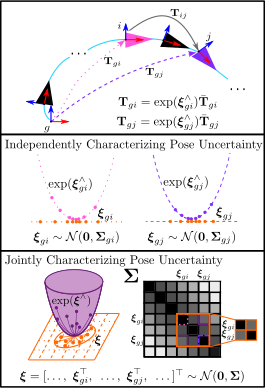
\includegraphics[width=0.9\columnwidth]{figures/main-example2.pdf}
    \caption{
    最先进的位姿图SLAM算法在每个时间步中估计机器人机体相对于固定坐标系的位姿(如上图中的 $i$ 和 $j$ ),分别用 $\mathbf{T}_{gi}$ 和 $\mathbf{T}_{gj}$ 表示。 
    在求解SLAM后,通常需要通过执行各种操作(如位姿组合、位姿求逆和相对位姿估计)来提取附加信息,同时精确地传播不确定性。
    本图顶部显示了一个相对位姿操作 $\mathbf{T}_{ij}$ 的示例。
    最近的研究已经表明,在特殊欧几里德群的李代数(如上图中所示)中,将不确定性作为高斯随机变量($\boldsymbol{\xi}_{gi}, \boldsymbol{\xi}_{gj}$)的刻画,会导致一致性的提高 \cite{barfoot2014associating};然而,这种方法的侧重于位姿组合,同时假设底层位姿是独立的。
    通常,从SLAM中估计的位姿高度相关 \cite{dissanayake2001a}。
    本文提出了一个在李代数空间中联合刻画一组相关位姿的不确定性的框架(如上图底部插图所示)。 
    然后描述了如何在此框架内执行位姿组合、位姿求逆和相对位姿操作。}
    \label{fig:main_example}
\end{figure}

\section{序言}

机器人位姿(位置和方向)不确定性的精确刻画对于鲁棒的长期的自主性至关重要,因为规划和安全决策通常基于它们的数值 \cite{thrun2005probabilistic}。例如,过于自信的位置估计可能导致自动驾驶汽车驶出车道或水下航行器与水下建筑相撞。另一方面,信心不足会导致行动迟缓。  

最早刻画坐标帧关系的位姿不确定性的论文之一,使用多元高斯参数向量和相关协方差矩阵来表示物体的相对位姿 \cite{smith1986a}。 
这篇论文后来被Smith、Self和Cheesman \cite{smith1990a} 扩展,将多个不确定的空间关系表示为一个可用于评估任意给定位姿相对于任意其它位姿的不确定性的随机映射(\textit{stochastic map})。 
他们还提出了几种操作(如 \figref{fig:main_example} 所示的相对位姿操作),这些操作能够提取不直接估计的附加信息,以及通过这些操作基于一阶坐标的方法传播不确定性。 
% These methods had a significant effect on the field and have been widely used since. 
为简洁起见,在文献 \cite{smith1990a} 中提出的操作通常由论文作者的首字母 (SSC) 表示。 



尽管众所周知,刚体变换(或 $\mathbb{R}^3$ 的运动群)是由三维(3D)特殊欧几里德群~\citep{spong2005robot,murray1994mathematical},$\mathrm{SE}(3)$ 描述的,这些变换的不确定性通常在局部坐标系中建模,从而导致在估计问题~\citep{huang2007convergence}中的不一致性或在不确定性传播~\citep{rodriguez2018importance}中的单调性损失。\citet{wang2008nonparametric} 和 \citet{long2013banana} 通过使用位于 $\mathrm{SE}(d)$ 的李代数中的指数坐标(\emph{exponential coordinates})来表示每个位姿,能够克服这些问题。 
 
\citet{barfoot2014associating} 证明了通过直接在李代数中对不确定性进行建模,然后使用指数映射在群空间中诱导分布,可以简化传播计算。 
由于李代数是一个向量空间,一个小的扰动项可以在 $\mathbb{R}^6$ 中建模为零均值高斯噪声,然后用于扰动群空间中的平均(或标称)位姿。 
文献 \cite{barfoot2014associating} 然后在此基础上,推导出当相关位姿独立时位姿组合操作的一阶和二阶不确定性传播。 
我们对一组位姿的不确定性进行建模的方法与此类似,但是我们放弃了独立性要求,因为由SLAM估计的位姿很少独立,并且它还附加描述了位姿求逆和相对位姿提取的附加操作(参见 \figref{fig:main_example})。 

本文的主要贡献如下:
\begin{enumerate}
    \item 我们提出了一个框架,描述了如何表示联合相关的位姿,同时使用李代数来刻画不确定性;
    \item 我们推导了所提议的框架与SSC操作的等价性;
    \item 我们描述了如何从替代的不确定性刻画参数化转换到所提议的框架(包括从MLE的解中提取李代数协方差);而且, 
    \item 我们发布了一个配套的C++库实现,以及这里介绍的例子。
\end{enumerate}
本文的其余部分组织如下:
第 \ref{sec:SE3} 节简要介绍了特殊欧几里德群及其在李群理论中的一些必要概念。 
第 \ref{sec:SSC} 节提供了SSC不确定性表示框架及其相关操作的摘要。 
第 \ref{sec:lie_joint_uncertainty} 节描述如何使用李代数来描述联合分布位姿的不确定性。 
第 \ref{sec:pose_composition}, \secref{sec:inverse}, 和 \secref{sec:relative_pose} 节分别描述了位姿组合、位姿求逆和相对位姿操作的推导,以及在李代数上不确定性的刻画。
第 \ref{sec:conversion} 节描述了如何从基于坐标系的不确定性表示转换为基于李代数的不确定性表示,以及如何从MLE的解中提取位姿不确定性的估计。
第 \ref{sec:eval} 节描述了所提议的方法的实验评估。
第 \ref{sec:library} 节描述了已发布的代码库的实现。 
最后, 第 \ref{sec:conclusion} 节总结全文。 
